\chapter{Marco Teórico}
% \section{Documentos Digitales}

%%%%
% Es importante en primer medida exponer las implicancias de los denominados 
% Documentos Digitales.



%%%%%%
% Seguidamente, es necesario definir lo que significaría validar un documento digital. 



% \section{Herramientas Tecnológicas para Validar Documentos Digitales}
%%%
Sin perjuicio de que existan diversas herramientas tecnológicas referentes o para validar documentos
digitales, a efectos del presente trabajo se expondrán el certificado digital y la Blockchain.

\section{Certificado Digital y Firma Digital}
Por un lado, el Certificado Digital es un documento emitido por una organización que presta un servicio (denominada autoridad de certificación), el 
documento o archivo digital contiene datos relacionado a un usuario en particular, una persona física o una organización. El certificado 
puede ser emitido en diversos formatos de archivos, la autoridad encargada reconoce y confirma los datos expuestos en el certificado 
digital, con utilización de técnicas criptográficas de clave pública y privada o de infraestructura de clave pública (Public key infrastructure) \cite[]{avila_implementacion_2015}.

La infraestructura de clave pública permite a las entidades ser autenticadas y reconocidas por otras entidades mediante los certificados 
digitales que además permiten cifrar y descifrar mensajes, firmar digitalmente y garantizar su integridad \cite[]{avila_implementacion_2015}. 

Las partes o componentes más importante de una \gls{pki} son las que se exponen a continuación \cite[]{avila_implementacion_2015}:

\begin{itemize}
    \item La \gls{ac}: encargada de generar, emitir y revocar los certificados; es la responsable que da  legitimidad a la clave pública con respecto a la  entidad. 

    \item La \gls{ra}: es la responsable de verificar si los enlace de las claves públicas corresponden a las entidades titulares.
    
    \item Los repositorios: se encargan de almacenar la información relativa a la \gls{pki}, como los repositorios que guardan las claves públicas y  otras que resguardan las listas de claves revocadas.

    \item La \gls{va}: se encarga de comprobar que los certificados digitales sean válidos.

    \item La \gls{tsa}: encargada de firmar los documentos para crear un registro específico en el momento exacto que existió.

    \item Los usuarios finales: obtienen una clave privada y una clave pública, también un certificado asociado a su clave pública. Mediante el uso de diversas aplicaciones hacen uso de la tecnología \gls{pki} para validar, cifrar y descifrar documentos.

\end{itemize}

Por otro lado, la Firma Digital es el mecanismo de criptografía de clave pública que permite dar
seguridad al receptor del documento firmado digitalmente; la firma digital se realiza con la
clave privada del remitente para cifrar la información a enviar y el receptor emplea la
clave pública del remitente para descifrarla, para así garantizar la autenticidad del origen de la informacion y verificar 
que ésta no fue modificada desde su creación. Este es un método para validar si mensajes, documentos o archivos han sido alterados.
Al método de clave pública y clave privada también se lo denomina método asimétrico \cite[]{avila_implementacion_2015}.


La aplicación del método de cifrado asimétrico puede encontrarse en el caso de que, por ejemplo,  una institución envía por correo electrónico un título digital a un estudiante. Es decir, 
la institución tiene en su poder
una clave pública y una privada,
la clave privada solo es conocida por la institución, ella no debe revelarla. Mientras
que la clave pública es un código que cualquier individuo puede conocerla, la institución puede 
mostrar su clave pública.
Para que el título tenga validez la institución utiliza su clave privada para cifrar el título digital. Una vez hecho esto, la institución envía el documento cifrado al estudiante y éste utiliza la llave pública para descifrar el documento y tener acceso al titulo digital.
El método valida inequívocamente a la institución ya que cualquier mensaje cifrado con la clave privada solamente puede ser descrifrado con la clave pública, por lo que ambas se complementan.
Por lo tanto si el mensaje es interceptado y cambian el  contenido, al momento de cifrarlo 
no podrá ser descifrado con la clave pública de la institución y de esta manera se verifica que la institución no envió el mensaje \cite[]{avila_implementacion_2015,garcia_rojas_implementacion_2008,avanzaexportador_certificados_2009}. 


Las autoridades certificadoras juegan un rol importante ya que ellas son la que emiten estas claves,
y validan la identidad de las organizaciones o personas. Por lo tanto si una entidad “A” quiere enviar un mensaje
privado a una entidad “B”, la entidad “A” debe consultar a la autoridad de certificación  es la clave pública de 
la entidad “B” y confiar que esa es la correcta \cite[]{garcia_rojas_implementacion_2008}. 

El cifrado asimétrico no es el único método pero es uno de los más comunmente utilizados para validar documentaciones digitales \cite[]{crypto_sheinix_bitcoin_2020}.  

Utilizando este método de criptografía se puede asegurar que una entidad es quién dice ser y también que un mensaje fue
emitido por ella. Por lo tanto el método de criptografía se utiliza para validar que una entidad es la que emitió un documento digital,
pudiendo ser este algún certificado académico,  título  académico \cite[]{avila_implementacion_2015,garcia_rojas_implementacion_2008,crypto_sheinix_bitcoin_2020}. 







  



\section{Conceptos de Interés}
Para mayor entendimiento sobre la temática del presente 
trabajo, se exponen a continuación determinados términos y 
conceptos que facilitarán la compresión sobre las tecnologías utilizadas para la validación de documentos digitales.

% Para una mayor comprensión,a continuación, se presentan los conceptos teóricos y tecnologías utilizadas en el desarrollo de la presente investigación.

% el "input"  incorpora los archivos sin salto de página.
% conceptos de interes
\subsection{Integridad}
Cuando utilizamos la palabra Integridad se hace referencia a que los datos no sufrieron ningún tipo de cambio o que los datos se mantuvieron constantes \cite[]{retamal_Blockchain_2017,badreddin_Blockchain_2018}.
\subsection{Documentos}
Los documentos son los  archivos o piezas documentales que necesitan de una validación para confirmar si sus datos son íntegros \cite[]{avila_implementacion_2015}. 

\subsection{Redes entre pares}
Las redes  con arquitectura entre iguales o Peer to Peer permite la conexión entre iguales o pares, donde cada usuario cumple el rol de servidor o de cliente, sin la necesidad de servidores centrales. 
Los datos están distribuidos dentro de la red de pares permite que los usuarios puedan acceder directamente a ella \cite[]{schollmeier_definition_2002}. 
\subsection{Protocolo de Consenso}

Son los protocolos que ejecutan los nodos de la red descentralizada para decidir qué bloques se van almacenar en la  Blockchain  y qué nodo es responsable de hacerlo
\cite[]{retamal_Blockchain_2017,badreddin_Blockchain_2018}.
\subsection{Función Hash}
% Función de resumen o función hash, es un proceso por el cual usa como entrada 
% una cantidad de datos variables de longitud no definida y de salida genera una cantidad de 
% datos variables de 
% longitud fija.

Función de resumen o función hash, es un algoritmo matemático  que usa como entrada 
una cantidad de datos variables de longitud no definida y de salida genera una cantidad de 
datos variables de longitud fija. Sin importar la los datos de entrada  la función siempre mantiene 
la misma longitud para los datos de salida. Unas de sus características importantes es la dificultad de  encontrar
la entrada de datos a partir de la salida, ya que el mínimo cambio en la entrada altera la salida \cite[]{drescher_Blockchain_2017,joaquin_lopez_lerida_economiBlockchain_2016}.

\subsection{Nodos}
Los nodos de una Blockchain, son los participantes de la red de una  Blockchain específica, donde cada uno almacenan los bloques y compiten
por agregar  nuevos y validar transacciones, los nodos contienen toda la información, si 
en algún momento todos los nodos de la red desaparecen, no existiría la  Blockchain en la que los nodos formaban parte.
A medida que el número de nodos de la red aumenta, también lo hará la descentralización y seguridad \cite[]{drescher_Blockchain_2017,nakamoto_bitcoin_2008,vazquez_episodio_2020}.
\subsection{ Prueba de Trabajo} \label{sec:pow}

La Prueba de Trabajo o Proof of Work (PoW) es un protocolo en el cual se le pide a un usuario o cliente que resuelva
un problema matemático que requiere de poder computacional, la complejidad de él determina el tiempo aproximado que se tarda en resolverlo.
En el caso de algunas  Blockchain usan este protocolo mediante el cálculo de hashes, en el cual deben
iniciar con una serie de ceros, por cada cero que inicie el hash el problema aumenta de manera exponencial \cite[]{nakamoto_bitcoin_2008,vazquez_episodio_2020,back_hashcash_2002}.


\subsection{Prueba de Participación }
La Prueba de Participación o Proof of Stake (PoS) es un protocolo de consenso como 
PoW pero, la idea de PoS es reducir los costos de consumo energético  producido por el 
poder computacional que se necesita con el protocolo de PoW \cite[]{vazquez_episodio_2020,brys_cadena_2019}.

En PoS  cuenta con la analogía en el que los nodos de la red deben tener una cantidad
de la moneda nativa de la  Blockchain bloqueada, como consecuencia, los nodos 
con más cantidad de monedas bloqueadas tienen más posibilidad de ser elegidos para validar el nuevo bloque \cite[]{vazquez_episodio_2020,brys_cadena_2019}.
 
Cuanta más \glspl{criptomoneda} tiene bloqueada el nodo, el incentivo en realizar 
actividades maliciosas en la red disminuye, porque algún  ataque que perjudique a  la 
red puede impactar en el valor de la moneda bajando su precio, por lo tanto la cantidad de dinero bloqueado
se traducen en pérdidas, por ende el incentivo que querer controlar la red completa se reduce, 
en cambio teniendo más cantidad de la criptomoneda nativa, tiene más posibilidades
de ser elegido como el nodo que forja el bloque y recibir la recompensa \cite[]{vazquez_episodio_2020,king_ppcoin_2012,academia_que_2018}.

\subsection{Prueba de Autoridad }\label{sec:poa}
La Prueba de Autoridad o Proof of Authority  (PoA) es el protocolo de consenso utilizado en redes  Blockchain  como la  Blockchain  Federal Argentina \cite[]{Blockchain_federal_argentina_protocolos_2020}.
% \footnote{\url{https://bfa.ar/}}.

La PoA funciona en una red entre pares donde se conoce la identidad de los nodos, que en comparación con el protocolo PoW no es necesario. 
Este protocolo brinda la ventaja de ejecutar un mayor número de transacciones en menos tiempo en comparación  a los protocolos PoW y PoS \cite[]{retamal_Blockchain_2017,Blockchain_federal_argentina_protocolos_2020}.
 
\subsection{Dirección}
Una dirección o address  es la clave pública de un usuario de la red o elemento de le red Blockchain, el cual se pueden utilizar como
dirección de destinatario en las transacciones, sirve para identificar a un  usuario permitiendo enviar la transacción,
es usada para encriptar la transacción y que pueda ser descifrada solamente por el poseedor de la clave privada correspondiente a la clave pública \cite[]{drescher_Blockchain_2017}.
\subsection{Billetera}
Una Billetera o Wallet es una herramienta de software que permite a los usuarios enviar y recibir
criptoactivos de manera relativamente sencilla, algunas también permiten interactuar con los smart contract,
se usan estas billeteras para hacer más sencillo la manera de comunicar con la Blockchain.
Un usuario con su misma clave privada puede usarla en cualquier billetera o wallet que soporte el software.
Existen diferentes tipos de billeteras \cite[]{dannen_introducing_2017,ambito_cuales_2021,rezaeighaleh_new_2019}:
\begin{enumerate}
\item Hardware wallet: Son billeteras que almacenen la clave privada y pública de manera física, similar 
a un pendrive se consideran una de las formas más seguras, porque no están conectadas directamente a internet.
\item Wallet Online: Las claves están almacenadas en un servidor.
\item Wallet Escritorio: Aplicaciones descargadas y ejecutadas desde el computador, donde se puede acceder
a los criptoactivos que se gestionan.
\item Paper Wallet:  Las claves publicas y privadas son almacenadas en un papel físico.
\end{enumerate}

Algunas de las Wallet que permiten gestionar sus criptosactivos son metamask, trezor (física), coinbase, entre otros \cite[]{dannen_introducing_2017,ambito_cuales_2021,coinsenda_tipos_2019}.
% Blockchain
\section{Blockchain}
\input{marco_teorico/Blockchain/Blockchain} 
\subsection{Solidity}
Solidity es un lenguaje de programación orientado a objetos influenciado  por
C++, Python y JavaScript utilizado para crear los contratos inteligentes en las máquinas virtuales de Ethereum,
esto permite realizar aplicaciones que se almacenan en la Blockchain, aplicar estructuras de controles, creación de clases y comunicaciones entre smart contracts \cite[]{dannen_introducing_2017,ethereum_solidity_nodate}.






\subsection{Contratos Inteligentes}
También llamados Smarts Contracts, son códigos de programas almacenados en la Blockchain
donde asegura que no podrá ser modificado, contiene funciones y variables
para resolver un problema específico. El contrato inteligente puede recibir y devolver datos. 
Para que los nodos verifiquen que un contrato inteligente fue correctamente ejecutado comprueban si los datos
de entrada devuelve el dato de salida propuesto por el primer nodo que resolvió el código.   
Por ende se ejecutarán de la misma manera \cite[]{Blockchain_federal_argentina_smart_2020,raskin_law_2017}.
Esto brinda la posibilidad de realizar cualquier tipo de aplicaciones y 
los consumidores no necesitan confiar en el programa, ya que tienen la libertad de visualizar las 
acciones del contrato antes de ejecutarlo \cite[]{Blockchain_federal_argentina_smart_2020}. 
\subsection{Ethereum}
Ethereum es una plataforma open source, que sirve para programar contratos inteligentes, 
  su diferencia con las primeras  Blockchain como Bitcoin  es que Ethereum 
 permite resolver cualquier problema computacional. Esta  Blockchain brinda
 la posibilidad  de crear cualquier programa,  almacenar   y ejecutarlos de manera descentralizada,  facilita la creación de nuevos activos digitales y aplicaciones.
Existen Blockchains de pruebas, en la cual el funcionamiento  es 
similar a la red principal, donde los desarrolladores pueden probar sus programas
y conseguir las criptomonedas de manera gratuita, para hacer sus controles en
esas testnet. Las redes de pruebas de Ethereum más conocidas son Ropsten
Rinkeby, Kovan, etc \cite[]{dannen_introducing_2017,vazquez_episodio_2020,torres_Blockchain_nodate,sadouskaya_adoption_2017}.



\section{Aplicación Descentralizada}

% \section{Aplicación Descentralizada ( Distributed Application o DApp)}
Las Aplicaciones Descentralizadas o Distributed Application (DApp) se ejecutan en una Blockchain,
un usuario con una dirección puede ejecutar métodos definidos en un programa almacenado
en la Blockchain, la lógica del programa dependerá del código
que diseñó el programador. En Ethereum se permite diseñar programas con
los smart contract, en el lenguaje de programación Solidity, 
el cual es ejecutado por una máquina virtual que permanece en el nodo.
Algunas DApps conocidas son UniSwap \footnote{\url{https://app.uniswap.org/}}   usada para intercambiar criptomonedas 
dentro de la Blockchain, Opensea mercado para compra y venta de criptoactivos
\cite[]{dannen_introducing_2017}.
Existen diferentes sitios para visualizar las diferentes aplicaciones de las  Blockchain como \href{https://www.dapp.com/}{Dapp.com} , \href{https://dappradar.com/}{DappRadar.com}
, entre otros.  
\subsection{OpenCerts}
OpenCerts  es una aplicación que permite a las entidades como escuelas, universidades, gestionen los certificados de sus alumnos
de manera segura y sin intermediarios utilizado la tecnología  Blockchain.
La aplicación no almacena los datos privados de los alumnos, sino que utilizan las claves públicas referenciadas a los usuarios. La función de las organizaciones o entidades es gestionar los certificados de los alumnos 
asociándolos a su clave pública. Los estudiantes pueden consultar, descargar y compartir 
sus certificados. El administrador valida que las entidades dadas de alta sean correctas \cite[]{opencerts_gestion_nodate}.

Funciona generando 
un código único a partir del certificado e información extra considerada como necesaria para validar el documento en el futuro, y luego se crea 
un archivo con extensión  “.opencerts”;
dicho archivo se carga al sitio web de OpenCerts y compara el contenido con el almacenado en la  Blockchain para verificar si existió el 
certificado en cuestión.
Para dar de alta los certificados usan el smart contract donde también crean los métodos para emitir o revocar un documento \cite[]{opencerts_frequently_nodate}.

\begin{figure}[H]
  \centering
  {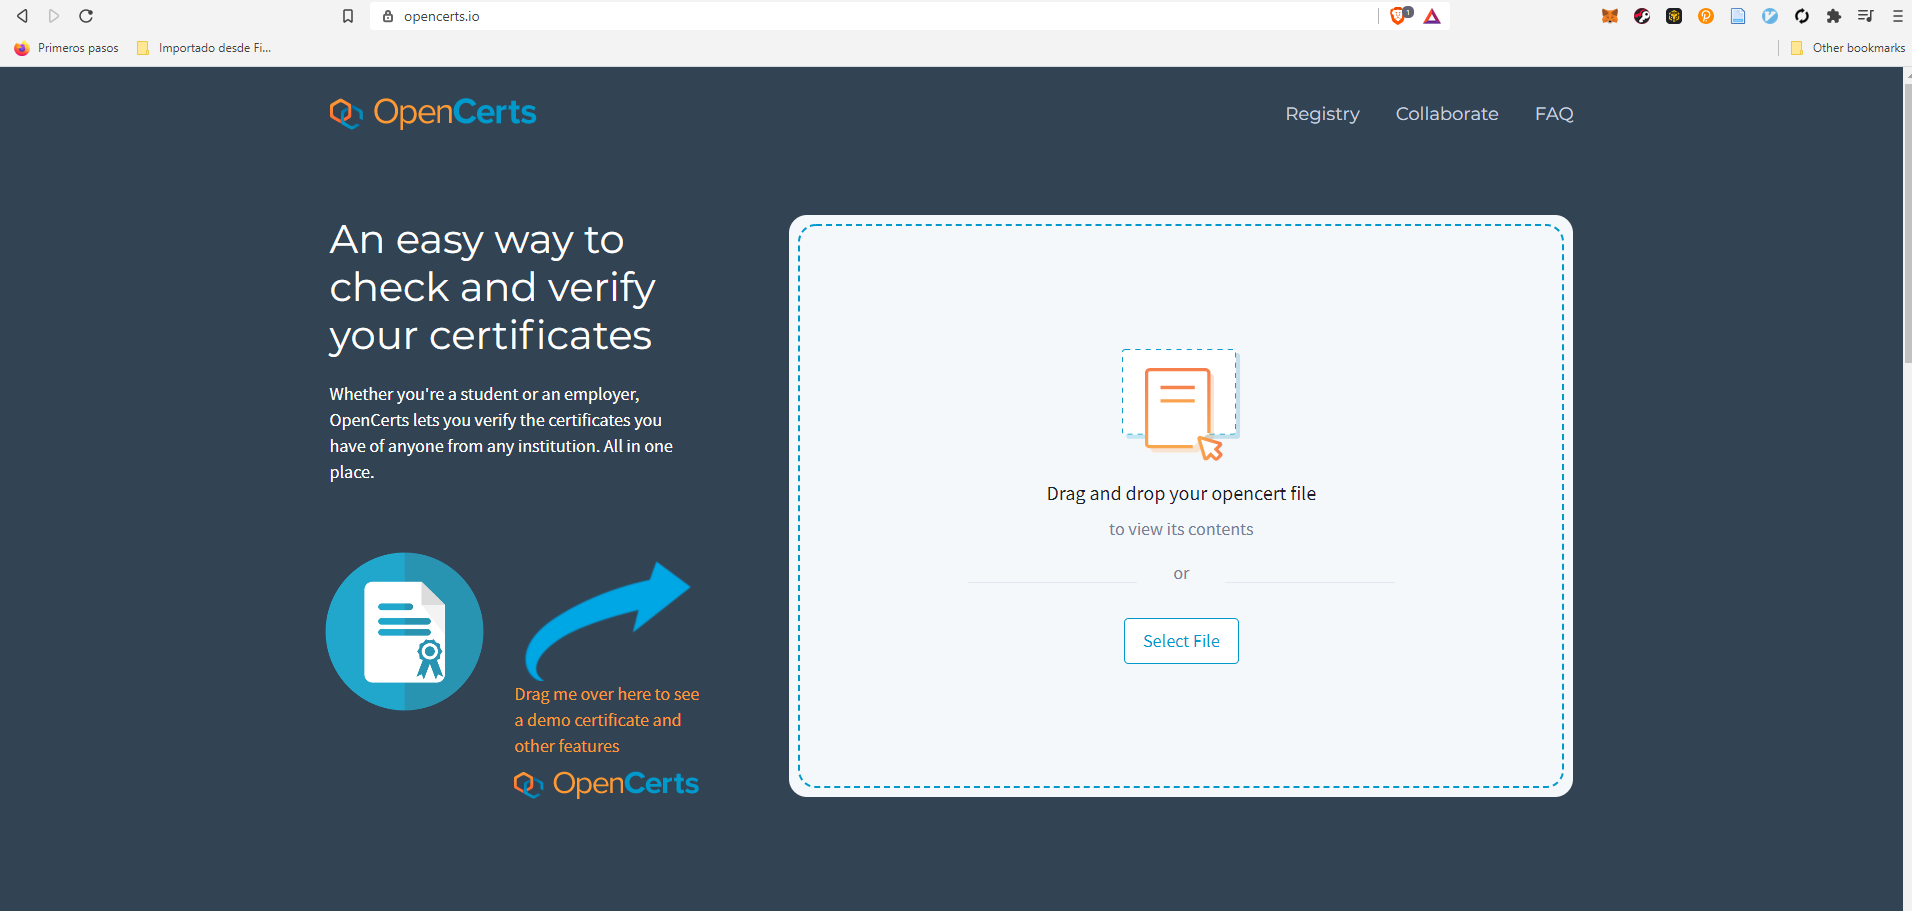
\includegraphics[scale=0.3]{OpenCerts_Home.png}}
  \caption{Página Web de OpenCerts}
  \label{img:opencerts_home}
\end{figure}

En la imagen \ref{img:opencerts_home} se puede observar lo sencillo que es verificar un documento. Simplemente se arrastra el  archivo 
de extensión“.opencerts”
y se buscará en la  Blockchain si realmente fue emitido por alguna entidad.
OpenCerts utiliza los smart contract en la  Blockchain de Ethereum. También utiliza tecnologías como Ract.js, Metamask, Web3.js, entre otros. 
Lo que permite desarrollar
un sistema de certificados totalmente descentralizado \cite[]{opencerts_gestion_nodate}. 
\subsection{BlockCerts}
Se define a si mismo 
como un estándar abierto   desarrollado por el MIT Media Lab y Learning Machine, para la construcción  de  aplicaciones que emiten y verifican registros oficiales basados
en la Blockchain. Pueden incluir certificados de registros civiles, académicos, licencias profesionales y más. 
Consiste en una librería con herramientas y apps móviles habilitando un ecosistema descentralizado, basado en estándar y habilitando verificación sin necesidad de la confianza mediante la tecnología  Blockchain \cite[]{blockcerts_introduction_nodate}.
Algunas universidades como el Instituto Tecnológico de Massachusetts (MIT), Tecnológico de Monterrey, la Universidad Harvard, la Universidad de California en Berkeley lo aplican. El 
estándar plantea que los certificados puedan ser compatibles a un nivel global, sin importar
la  Blockchain que se utilice pudiendo ser Bitcoin, Ethereum u otra \cite[]{edublocs_nueve_2019,criptomonedas_tv_entrevista_2018}. 

\begin{figure}[H]
  \centering
  {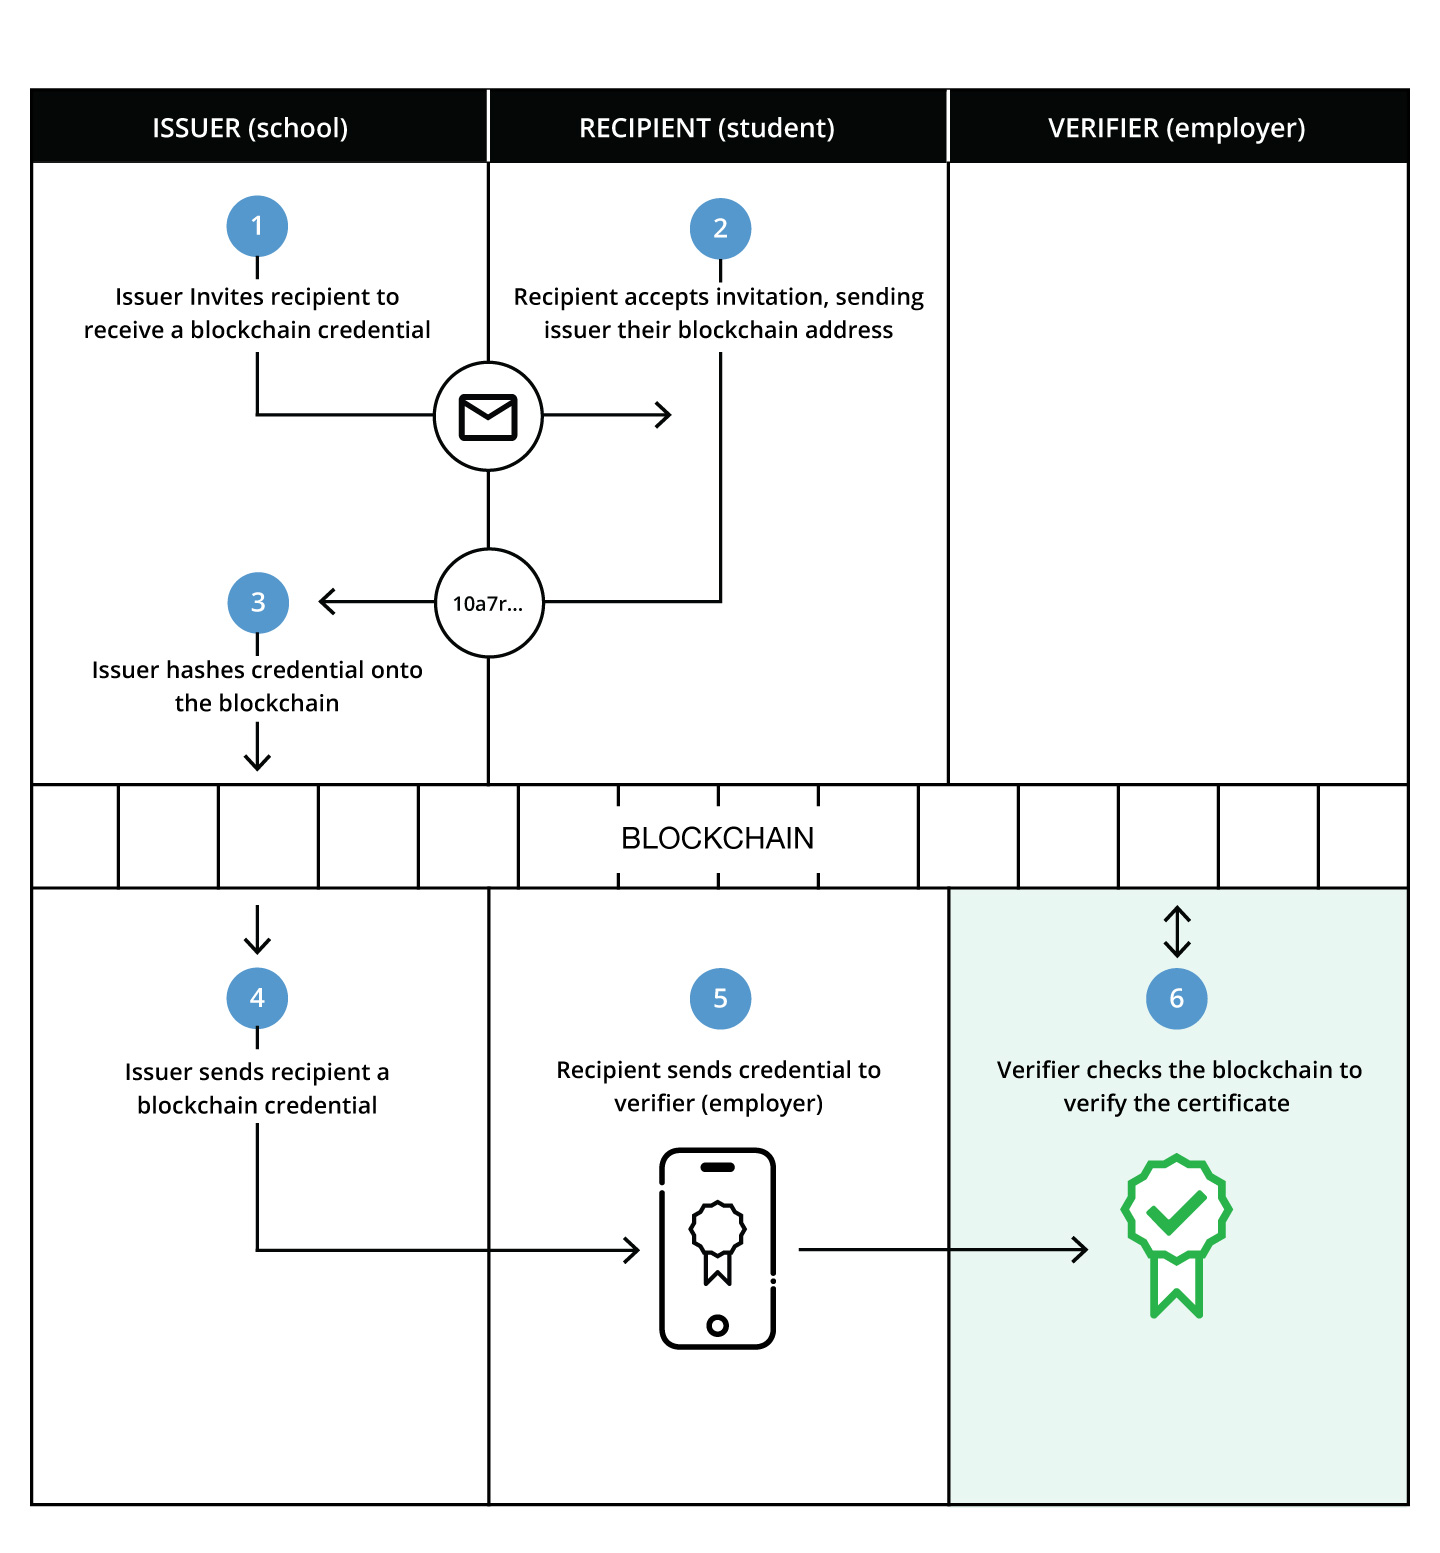
\includegraphics[scale=0.3]{blockcerts_how_it_works.jpg}}
  \caption{Imagen extraída de la página oficial de BlockCerts}
  \label{img:blockcerts_how_it_works}
\end{figure}

El flujo básico que se visualiza en  la figura \ref{img:blockcerts_how_it_works}   para comprobar que
un certificado se encuentra almacenado en la  Blockchain y es validado por un instituto se explica a continuación:

En el paso 1, el emisor o institución invita a un usuario a que brinde su dirección de cuenta o su clave pública creada 
descargando, la aplicación movil que provee BlockCerts. En el paso 2, el usuario envía al emisor su clave pública.
El paso 3 y 4, el emisor crea el hash a partir del certificado y lo almacena en la  Blockchain para luego enviar un archivo de tipo JSON 
\footnote{JavaScript Object Notation es un formato basado en texto estándar para representar datos estructurados \cite[]{mozilla_trabajando_json}.}, que contiene
la información sobre el documento del estudiante o dueño del certificado. En el paso 5, puede enviar este documento a cualquier empresa o individuo que desee.
 En el paso 6 el usuario que posee el archivo puede verificarlo en el sitio web de  BlockCerts \cite[]{blockcerts_introduction_nodate}.

 



